\section{实体-关系图}

\begin{figure}[H]
    \centering
    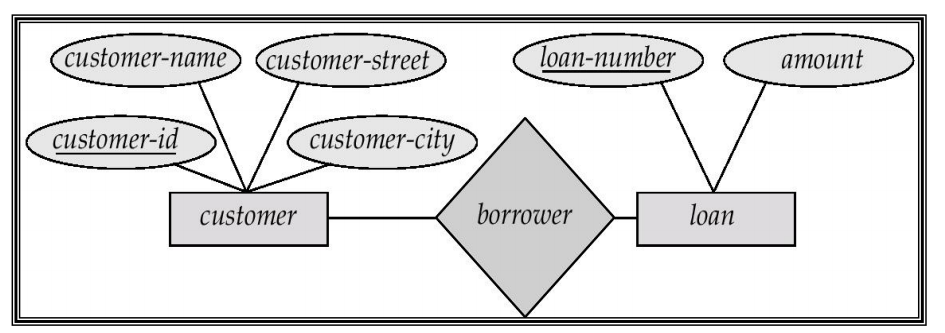
\includegraphics[width=0.8\linewidth]{image1.png}
    \caption{}
    \label{}
\end{figure}

\begin{figure}[H]
    \centering
    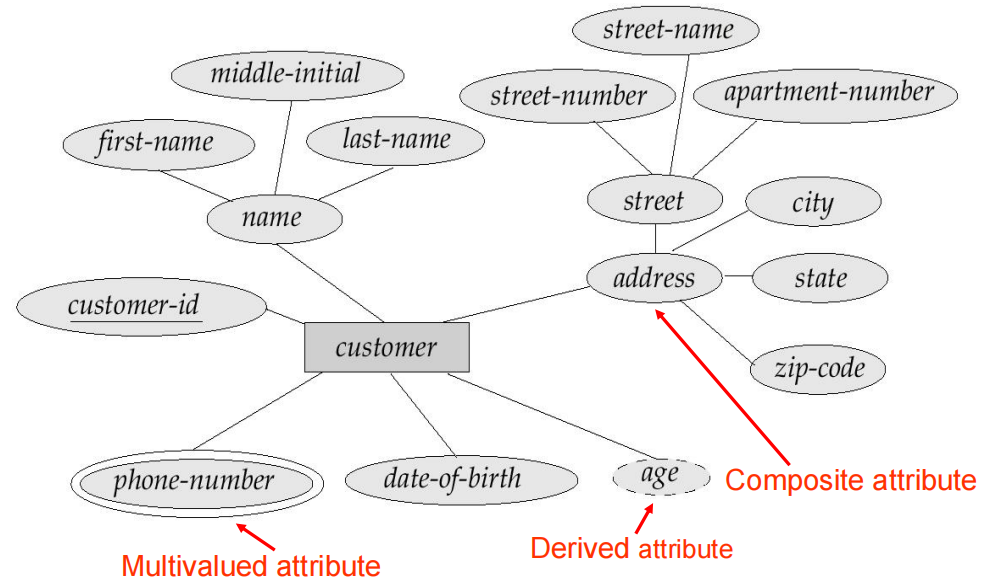
\includegraphics[width=0.8\linewidth]{image2.png}
    \caption{}
    \label{}
\end{figure}

\begin{itemize}
    \item 矩形表示Entity Set
    \item 菱形表示Relationship Set
    \item 线条将属性与实体集相连,将实体集与关系集相连。
    \item 椭圆表示属性:双椭圆表示多值属性;虚线椭圆表示派生属性。
    \item 下划线表示主键属性。
\end{itemize}

一个关系的实体集不必是不同的,例如,自环联系集。

Role:实体在关系中所起的作用,例如,label "manager" and "employee"被称为role;它们指定了员工实体如何通过"为...工作"关系集进行交互。

角色标签是可选的,用于阐明关系的语义。

我们通过在关系集和实体集之间绘制有向线($\to$)(表示"一个")或无向线(-)(表示"多个")来表达基数约束。

实体集在关系集中的参与情况:全参与(用双线表示):实体集中的每个实体至少参与关系集中的一个关系。

部分参与:某些实体可能不参与关系集中的任何关系。

映射基数约束限定了一个实体与发生关联的另一端实体可能关联的数目上限。

一般来说,任何非二元关系都可以通过创建一个人工实体集,用二元关系来表示。用一个实体集$E$和
三个新的关系集来替换实体集$A,B$和$C$之间的非二元关系$R$。
\begin{itemize}
    \item 为$E$创建一个特殊的标识属性
    \item 将$R$的任何属性添加到$E$中
    \item 对于$R$中的每个关系$(a_i,b_i,c_i)$,创建$R_A,R_B,R_C$
\end{itemize}